\chapter{Diseño de la interfaz de usuario}\label{chapter:diu}

A nivel de diseño de la interfaz, lo principal es reseñar que nos encontramos con una gran limitación: no podemos desarrollar una interfaz totalmente a nuestro gusto\footnote{El 16 de abril de 2022, la API para bots de Telegram fue actualizada\cite{telegramWebappUpdate} con una nueva función para abrir una aplicación web sin salir del bot como respuesta a varios eventos. Sin embargo, esa opción se ha descartado para este trabajo ya que la implementación del bot se encontraba en estado avanzado y se ha analizado que las complicaciones técnicas de implementar esta nueva interfaz extenderían el tiempo de desarrollo considerablemente. Se propone como mejora futura.}, sino que debemos usar la API que nos proporciona Telegram.

Es decir, \textbf{Mordente bot} va a operar dentro de un chat, y como todo chat, la interfaz estará compuesto sola y únicamente por mensajes, que podrán ser de distinto tipo (texto, imágenes, documentos, stickers...). La única adición que aporta Telegram a esta interfaz es que los mensajes que envía el bot pueden adjuntar un menú de opciones que el usuario puede pulsar para pedir al bot una determinada acción, además de tener un menú de comandos disponible continuamente junto al cuadro de introducción de texto.

Esta rigidez de la interfaz puede ser vista de manera positiva, ya que aporta las siguientes ventajas:

\begin{itemize}
    \item Las decisiones de diseño son mucho más simples, puesto que no tenemos todo un elenco de estilos, formatos e interacciones que elegir. Por ejemplo, si el usuario quiere acceder a la información general sobre la aplicación, la mejor solución dentro del bot es que el usuario use un comando \texttt{/about} al cual el bot responde con un texto explicativo. En el caso de una aplicación web, la interacción por parte del usuario podría ser desde pulsar un botón hasta usar un atajo de teclado, y la visualización podría ser desde sobreponer un cuadro con la información hasta enlazar a una página distinta.
    \item La personalización ya está implementada para nosotros: esta característica se delega a la propia aplicación de Telegram, que permite seleccionar el tema claro u oscuro o cambiar el tamaño del texto.
    \item La accesibilidad está garantizada, ya que la interfaz de mensajes ya está totalmente adaptada a personas con discapacidad auditiva o visual.
    \item La familiarización del usuario con la interfaz es mayor de antemano, ya que con toda probabilidad habrá usado un chat antes y la interfaz del bot no es más que una extensión de un chat corriente. Esto le supondrá una adaptación más sencilla y más centrada en saber cuál es la funcionalidad que en cómo está dispuesta.
    \item El usuario interacciona de forma privada en un chat con el bot, de modo que el tono de respuesta del bot y el intercambio de mensajes hacen que el usuario perciba la interfaz como más amigable y cercana.
    \item Los entornos que más necesitan la comunicación se benefician de esta integración. Por ejemplo, en el caso que nos ocupa siempre se suele usar un grupo de mensajería, y un bot puede ser integrado en un grupo de Telegram.
\end{itemize}

Decimos que la limitación es autoimpuesta porque es tarea de este trabajo también analizar si las ventajas expuestas superan o igualan a las desventajas de operar dentro de un chat, es decir, si un bot de Telegram de este tipo puede operar sin la ayuda de una aplicación web o móvil que la acompañe. Dicho de otra forma, se pretende aprovechar esta oportunidad para analizar las interacciones humano-chat como parte de los objetivos de este trabajo.


\subsection{Bocetos de interfaz}

Con todo lo anterior en mente, pasamos a crear varios bocetos de lo que debería ser la interfaz entre el usuario y el bot: uno para listar elementos, un segundo para mostrar el detalle de un elemento y un tercero para crear un elemento nuevo.

\subsubsection{Lista de elementos}

Aunque se ha expuesto que la interfaz está limitada a la API disponible, en el caso de las listas tenemos 3 opciones si queremos que el usuario pueda acceder al detalle de cada elemento:
\begin{enumerate}
    \item Enviar un mensaje muy corto acompañado de un menú, cada botón del menú muestra el título de un elemento y al pulsar en él se recibe el detalle.
    \item Igual que la opción 1, pero añadiendo en el texto una lista de los elementos con un resumen de cada uno.
    \item Nueva opción explorada en este trabajo como variación de la opción 2: omitir el menú para no repetir los nombres, y en su lugar acompañar cada elemento de la lista con un comando del estilo \texttt{/event\_N} de manera que al pulsar y enviar el comando el bot responda con el detalle del elemento.
\end{enumerate}

En todo caso la lista debe ir acompañada de un botón para añadir elementos.

El diseño se ve en la figura \ref{fig:disenyo_lista}.

\begin{figure}[h]
\centering
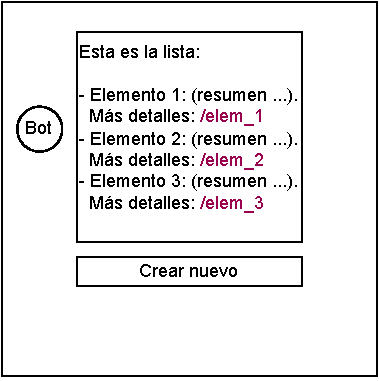
\includegraphics[width=0.5\textwidth]{imagenes/disenyo_interfaz/lista.drawio.pdf}
\caption{Diseño de la interfaz de lista}
\label{fig:disenyo_lista}
\end{figure}

\subsubsection{Detalle de elemento}

En este caso, toda la información sobre el elemento se muestra en el mensaje de respuesta, que va acompañado de un menú con las acciones que se pueden realizar con el elemento. Ver figura \ref{fig:disenyo_detalle}.

\begin{figure}[h]
\centering
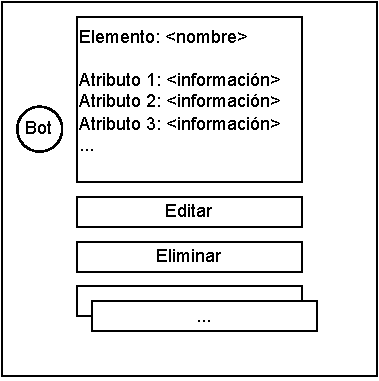
\includegraphics[width=0.5\textwidth]{imagenes/disenyo_interfaz/detalle.drawio.pdf}
\caption{Diseño de la interfaz del detalle de un elemento}
\label{fig:disenyo_detalle}
\end{figure}

\subsubsection{Creación de elemento}

La interfaz más sencilla y equivalente a un formulario para crear un elemento es una conversación: el bot va preguntando cada campo requerido al usuario, que puede saltar los campos opcionales mediante un botón de \texttt{Saltar}.
Idealmente, para la introducción de fechas se debería mostrar un menú con forma de calendario. Ver figura \ref{fig:disenyo_creacion}.

\begin{figure}[h]
\centering
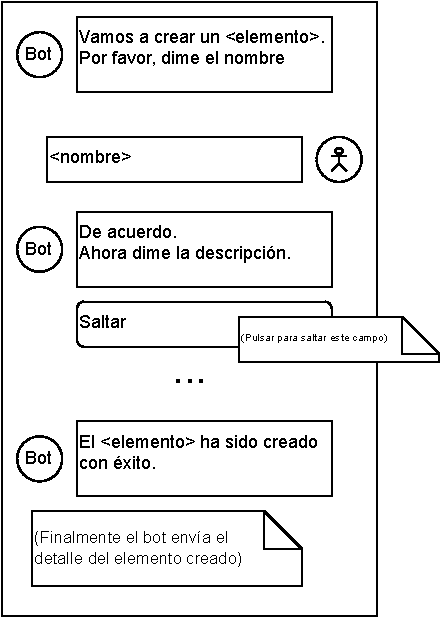
\includegraphics[width=0.5\textwidth]{imagenes/disenyo_interfaz/creacion.drawio.pdf}
\caption{Diseño de la interfaz de creación de un elemento}
\label{fig:disenyo_creacion}
\end{figure}

\section{Imagen de marca}

Para que la marca \textbf{Mordente} sea reconocible por los usuarios ya activos y los potenciales usuarios, vamos a definir tres elementos básicos: tipografía, logotipo y paleta de colores.

\subsection{Tipografía}

Para el logotipo hemos escogido la tipografía \textbf{Eczar} debido a su parecido con la mayoría de tipografías utilizadas para la edición de partituras.

El resto de la aplicación utilizará la tipografía por defecto del sistema, ya que esto es controlado por \textbf{Telegram}. La \textit{landing page} reproducirá este mismo comportamiento, de modo que todo el contenido excepto el logotipo utilizará la tipografía nativa del sistema.

\subsection{Logotipo}

El logotipo usará un color \textbf{negro piano} (\#000000) con símbolo \textbf{blanco} (\#FFFFFF).

Se compondrá del texto \textbf{mordente} en la tipografía escogida y un símbolo de mordente a la izquierda sobre el texto, ligeramente sobresaliendo por la izquierda del espacio que ocupa el texto.

Podemos ver el imagotipo (compuesto por el símbolo y el texto) en la figura \ref{fig:imagotipo}. El isotipo, compuesto solo por el símbolo y usado cuando se dispone de menos espacio, se puede ver en la figura \ref{fig:isotipo}.

\begin{figure}[]
\minipage{0.5\textwidth}
  \centering
  
\includegraphics[width=0.7\linewidth]{imagenes/logo_mordente.pdf}
  \caption{Imagotipo de \textbf{Mordente}}\label{fig:imagotipo}
\endminipage\hfill
\minipage{0.5\textwidth}%
  \centering
  
\includegraphics[width=0.7\linewidth]{imagenes/isotipo_mordente.pdf}
  \caption{Isotipo de \textbf{Mordente}}\label{fig:isotipo}
\endminipage
\end{figure}

\subsection{Paleta de colores}

Crearemos una paleta de colores usando la herramienta \texttt{coolors.co} (\url{https://coolors.co}) que nos permite encontrar colores complementarios fácilmente.

Tras decidir entre varias alternativas, la paleta generada se puede observar en la figura \ref{fig:paletaMordente}.

Por un lado tendremos los dos colores del logotipo: negro piano y blanco puro, a los que añadiremos el rojo ``Rubí Antiguo'' como color primario y el color naranja ``Mandarina'' como color secundario:

\begin{itemize}
    \item El \textbf{rojo ``Rubí Antiguo''} (\#832232) imita al color de la madera los instrumentos de cuerda frotada.
    \item El \textbf{naranja ``Mandarina''} (\#EF8354) complementa al color primario añadiendo más cantidad de amarillo.
\end{itemize}



\begin{figure}[h]
\centering
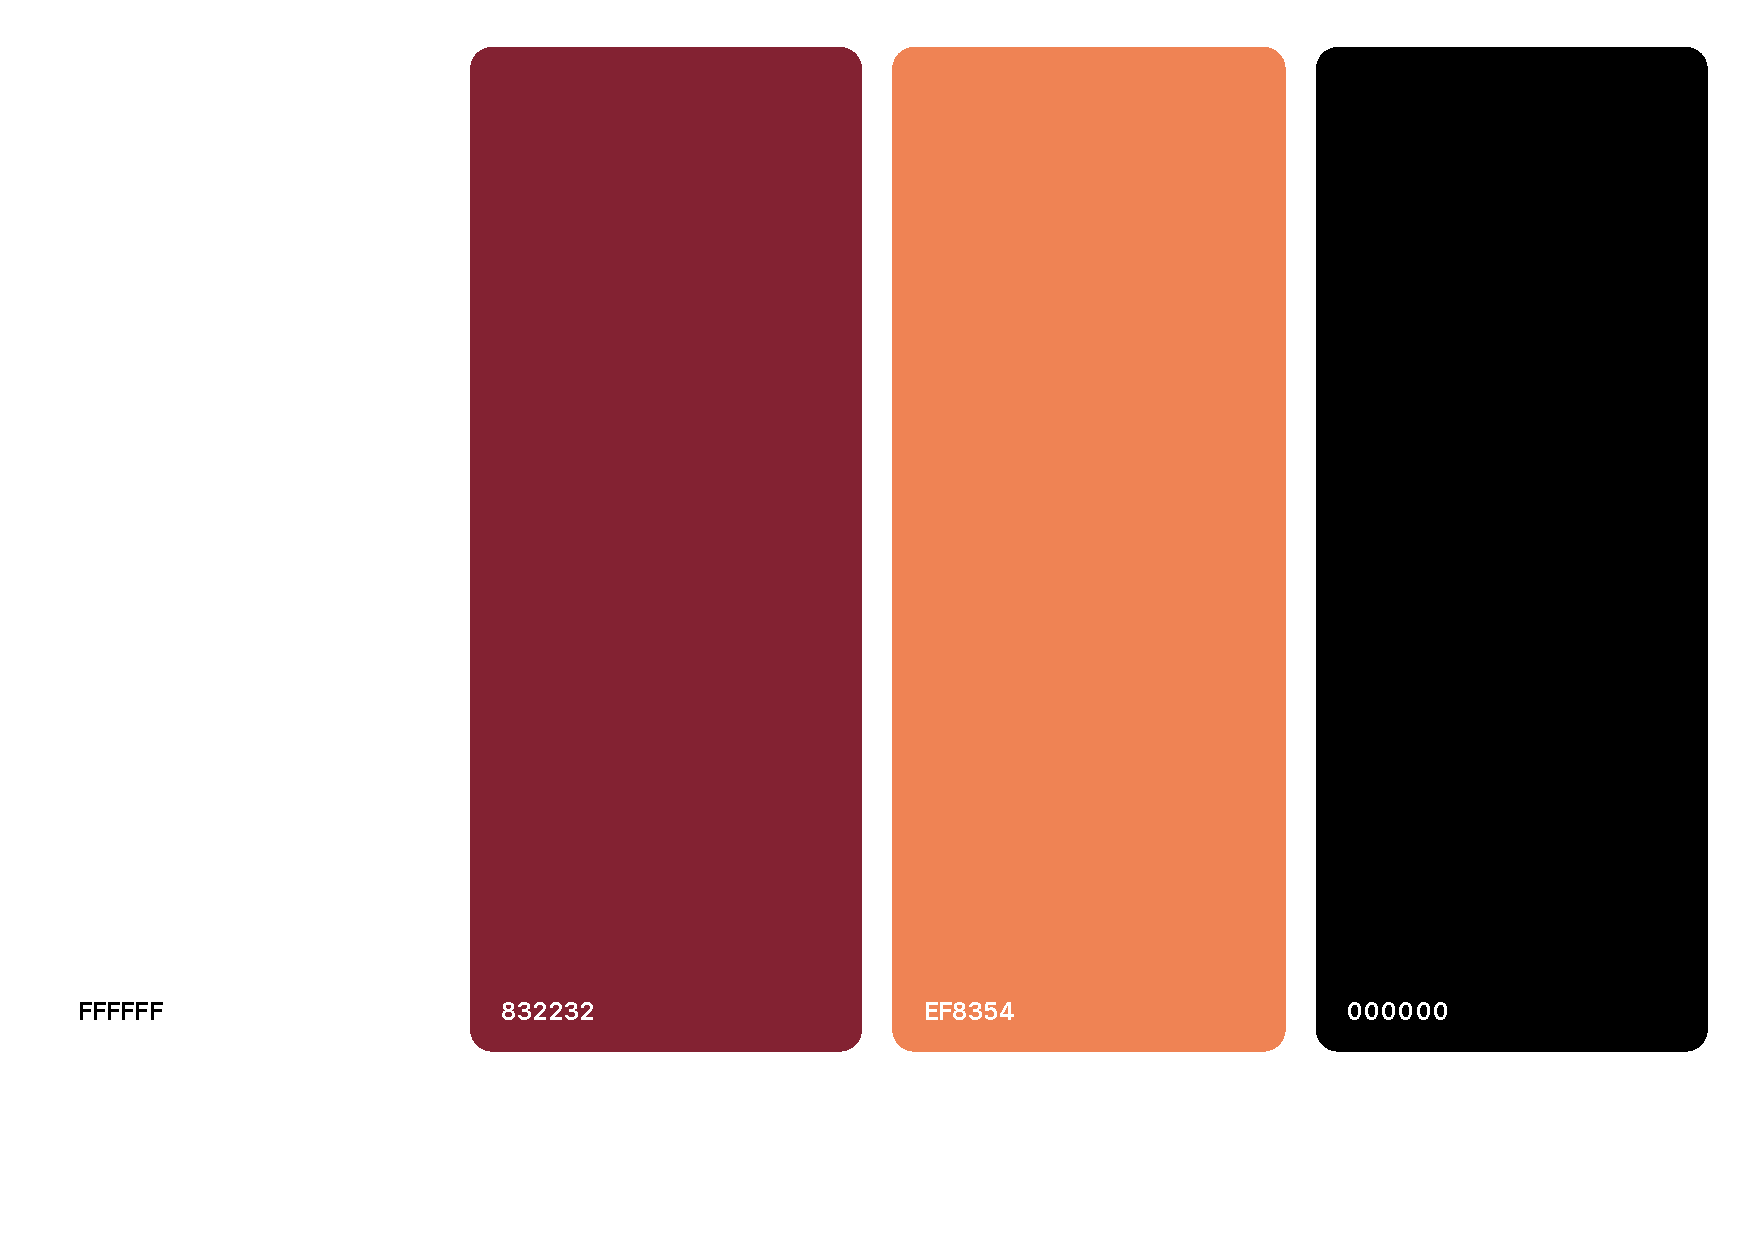
\includegraphics[width=\textwidth]{imagenes/disenyo_interfaz/mordente_paleta.pdf}
\caption{Paleta de colores}
\label{fig:paletaMordente}
\end{figure}
